\documentclass[11pt,compress,t,notes=noshow, xcolor=table]{beamer}

\input{../../style/preamble}
\input{../../latex-math/basic-math}
\input{../../latex-math/basic-ml}


\title{Applied Machine Learning}
% \author{LMU}
%\institute{\href{https://compstat-lmu.github.io/lecture_iml/}{compstat-lmu.github.io/lecture\_iml}}
\date{}

\begin{document}

\titlemeta{
Feature Engineering:
}{
Target Transformations
}{
figure/01_target_log_distribution
}{
\item Why and when to transform the target
\item Common transformations: log, Box-Cox, Yeo-Johnson
\item The transform-fit-invert pipeline
}


\begin{vbframe}{Why Transform the Target?}
Previous slides transformed \emph{features} ($\xv$); here we transform the \emph{target} ($y$). Predictions must then be inverted to the original scale.
\vfill
When targets are heavily skewed, regression models struggle: large tail residuals dominate squared-error loss, error variance grows with $y$ (heteroscedasticity), and the model ``chases'' extremes.
\begin{center}
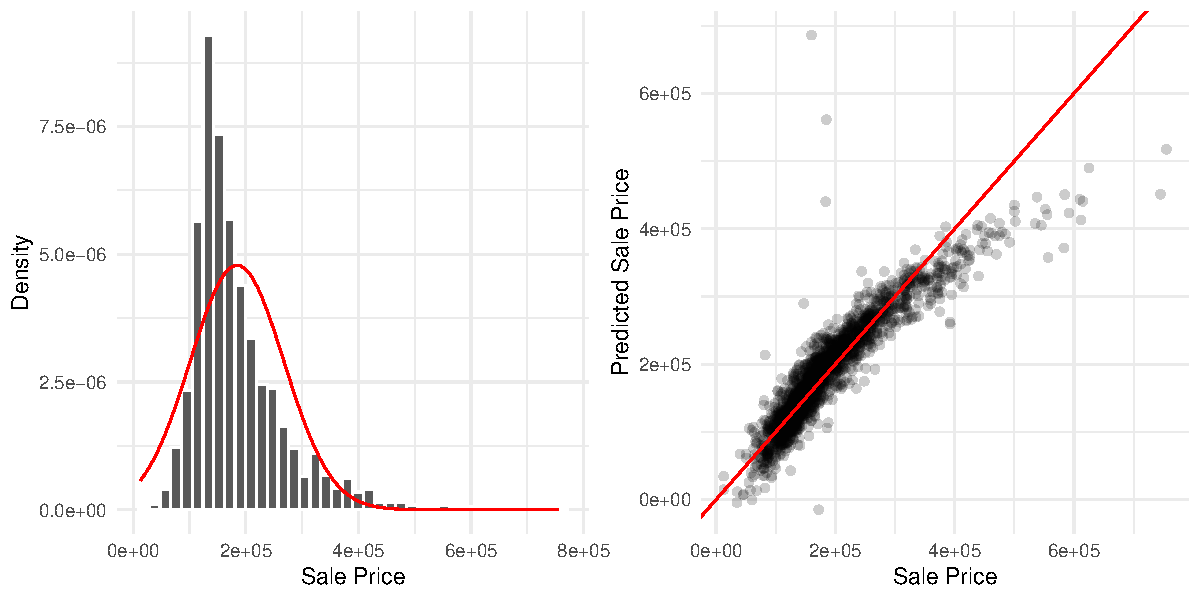
\includegraphics[width=0.65\textwidth]{figure/01_target_original_distribution.pdf}
\end{center}
\vspace{-0.5em}
\footnotesize
Ames housing data: sale prices are right-skewed (left). Predictions of a linear model fit poorly at the extremes (right) because tail residuals dominate the squared-error loss.
\end{vbframe}


\begin{vbframe}{Log Transformation}
The simplest fix: model $\log(y)$ instead of $y$, then exponentiate predictions back.
\begin{columns}[T]
\begin{column}{0.55\textwidth}
\vspace{0.3em}
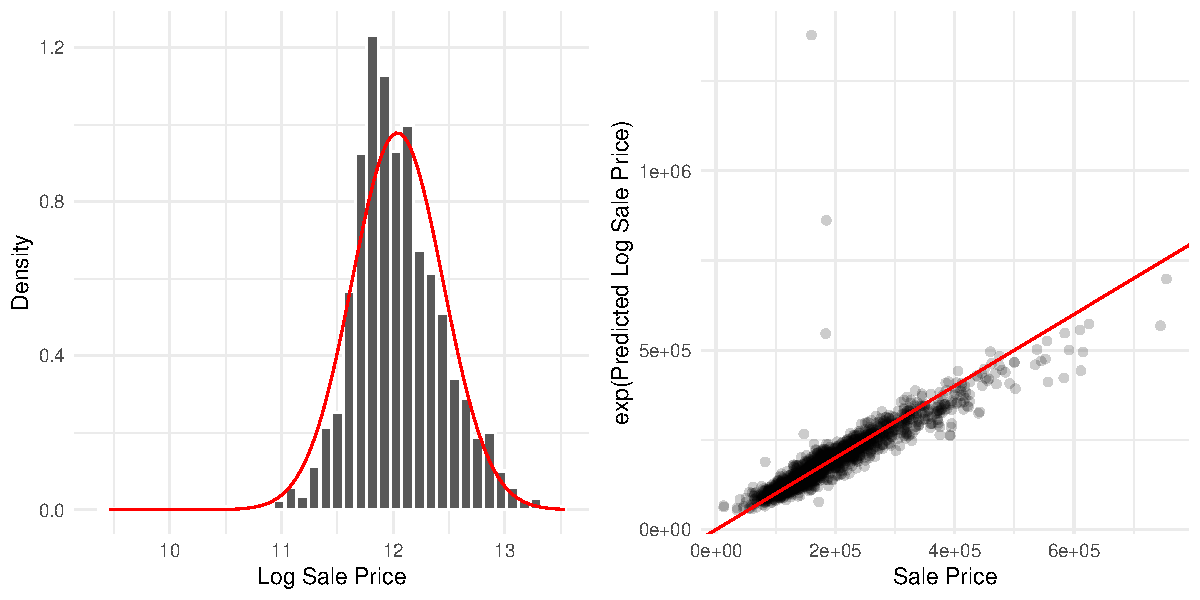
\includegraphics[width=\textwidth]{figure/01_target_log_distribution.pdf}
\end{column}
\begin{column}{0.43\textwidth}
\vspace{0.3em}
\footnotesize
\textbf{Why it works:} the log compresses the long right tail, making the error distribution more symmetric and stabilizing its variance.

\vspace{0.5em}
\normalsize
\textbf{Variants:}
\begin{itemize}\setlength{\itemsep}{2pt}
    \item $\log(y)$ -- requires $y > 0$
    \item $\log(y + 1)$ -- handles zeros (common for count data)
    \item $\log(y + c)$ -- shift by constant $c$ for negative or zero $y$
\end{itemize}
\end{column}
\end{columns}
\end{vbframe}


\begin{vbframe}{The Transform-Fit-Invert Pipeline}
\vfill
Target transformations are \textbf{not} a preprocessing step -- they are part of the model:
\vfill
\begin{enumerate}\setlength{\itemsep}{4pt}
    \item \textbf{Transform} the target: $\tilde{y} = f(y)$ \quad (e.g., $f = \log$)
    \item \textbf{Fit} the model on transformed targets: $\hat{\tilde{y}} = g(\xv)$
    \item \textbf{Invert} predictions back to the original scale: $\hat{y} = f^{-1}(\hat{\tilde{y}})$
\end{enumerate}
\vfill
\textbf{Important:} the transformation parameters (e.g., $\lambda$ for Box-Cox) must be estimated on the \textbf{training fold only}. Fitting the transformation on the full dataset before splitting leaks information and produces overly optimistic CV results.
\vfill
\footnotesize
In scikit-learn: wrap with \texttt{TransformedTargetRegressor(regressor, func=..., inverse\_func=...)}\\
In R/mlr3: use \texttt{PipeOpTargetTrafo} inside a pipeline (see time series chapter for a worked example)
\vfill
\end{vbframe}


\begin{vbframe}{Power Transforms: Box-Cox and Yeo-Johnson}
\vfill
Instead of choosing $\log$ by hand, power transforms find the best transformation automatically by optimizing a parameter $\lambda$:
\vfill
\begin{columns}[T]
\begin{column}{0.48\textwidth}
\textbf{Box-Cox} (requires $y > 0$):
$$y^{(\lambda)} = \begin{cases}
\dfrac{y^\lambda - 1}{\lambda} & \lambda \neq 0 \\[6pt]
\log(y) & \lambda = 0
\end{cases}$$
\end{column}
\begin{column}{0.48\textwidth}
\textbf{Yeo-Johnson} (any $y$):
\scriptsize
$$y^{(\lambda)} = \begin{cases}
\dfrac{(y{+}1)^\lambda - 1}{\lambda} & \lambda \neq 0,\, y \geq 0 \\[2pt]
\log(y{+}1) & \lambda = 0,\, y \geq 0 \\[2pt]
-\dfrac{(-y{+}1)^{2-\lambda} - 1}{2-\lambda} & \lambda \neq 2,\, y < 0 \\[2pt]
-\log(-y{+}1) & \lambda = 2,\, y < 0
\end{cases}$$
\normalsize
\end{column}
\end{columns}
\begin{itemize}\setlength{\itemsep}{2pt}
    \item $\lambda$ is fit via maximum likelihood; Box-Cox special cases: $\lambda=1$ (identity), $0$ (log), $0.5$ ($\sqrt{y}$), $-1$ ($1/y$)
    \item \textbf{Decision rule:} use Box-Cox when $y > 0$ is guaranteed, Yeo-Johnson otherwise
\end{itemize}
\footnotesize
scikit-learn: \texttt{PowerTransformer(method='yeo-johnson'|'box-cox')}; R: \texttt{recipes::step\_BoxCox()}, \texttt{step\_YeoJohnson()}
\end{vbframe}


% TODO: regenerate this figure as PDF using mlr3 (current R script uses deprecated mlr)
\begin{vbframe}{Benchmark: Does It Help?}
\begin{columns}[T]
\begin{column}{0.52\textwidth}
\vspace{0.2em}
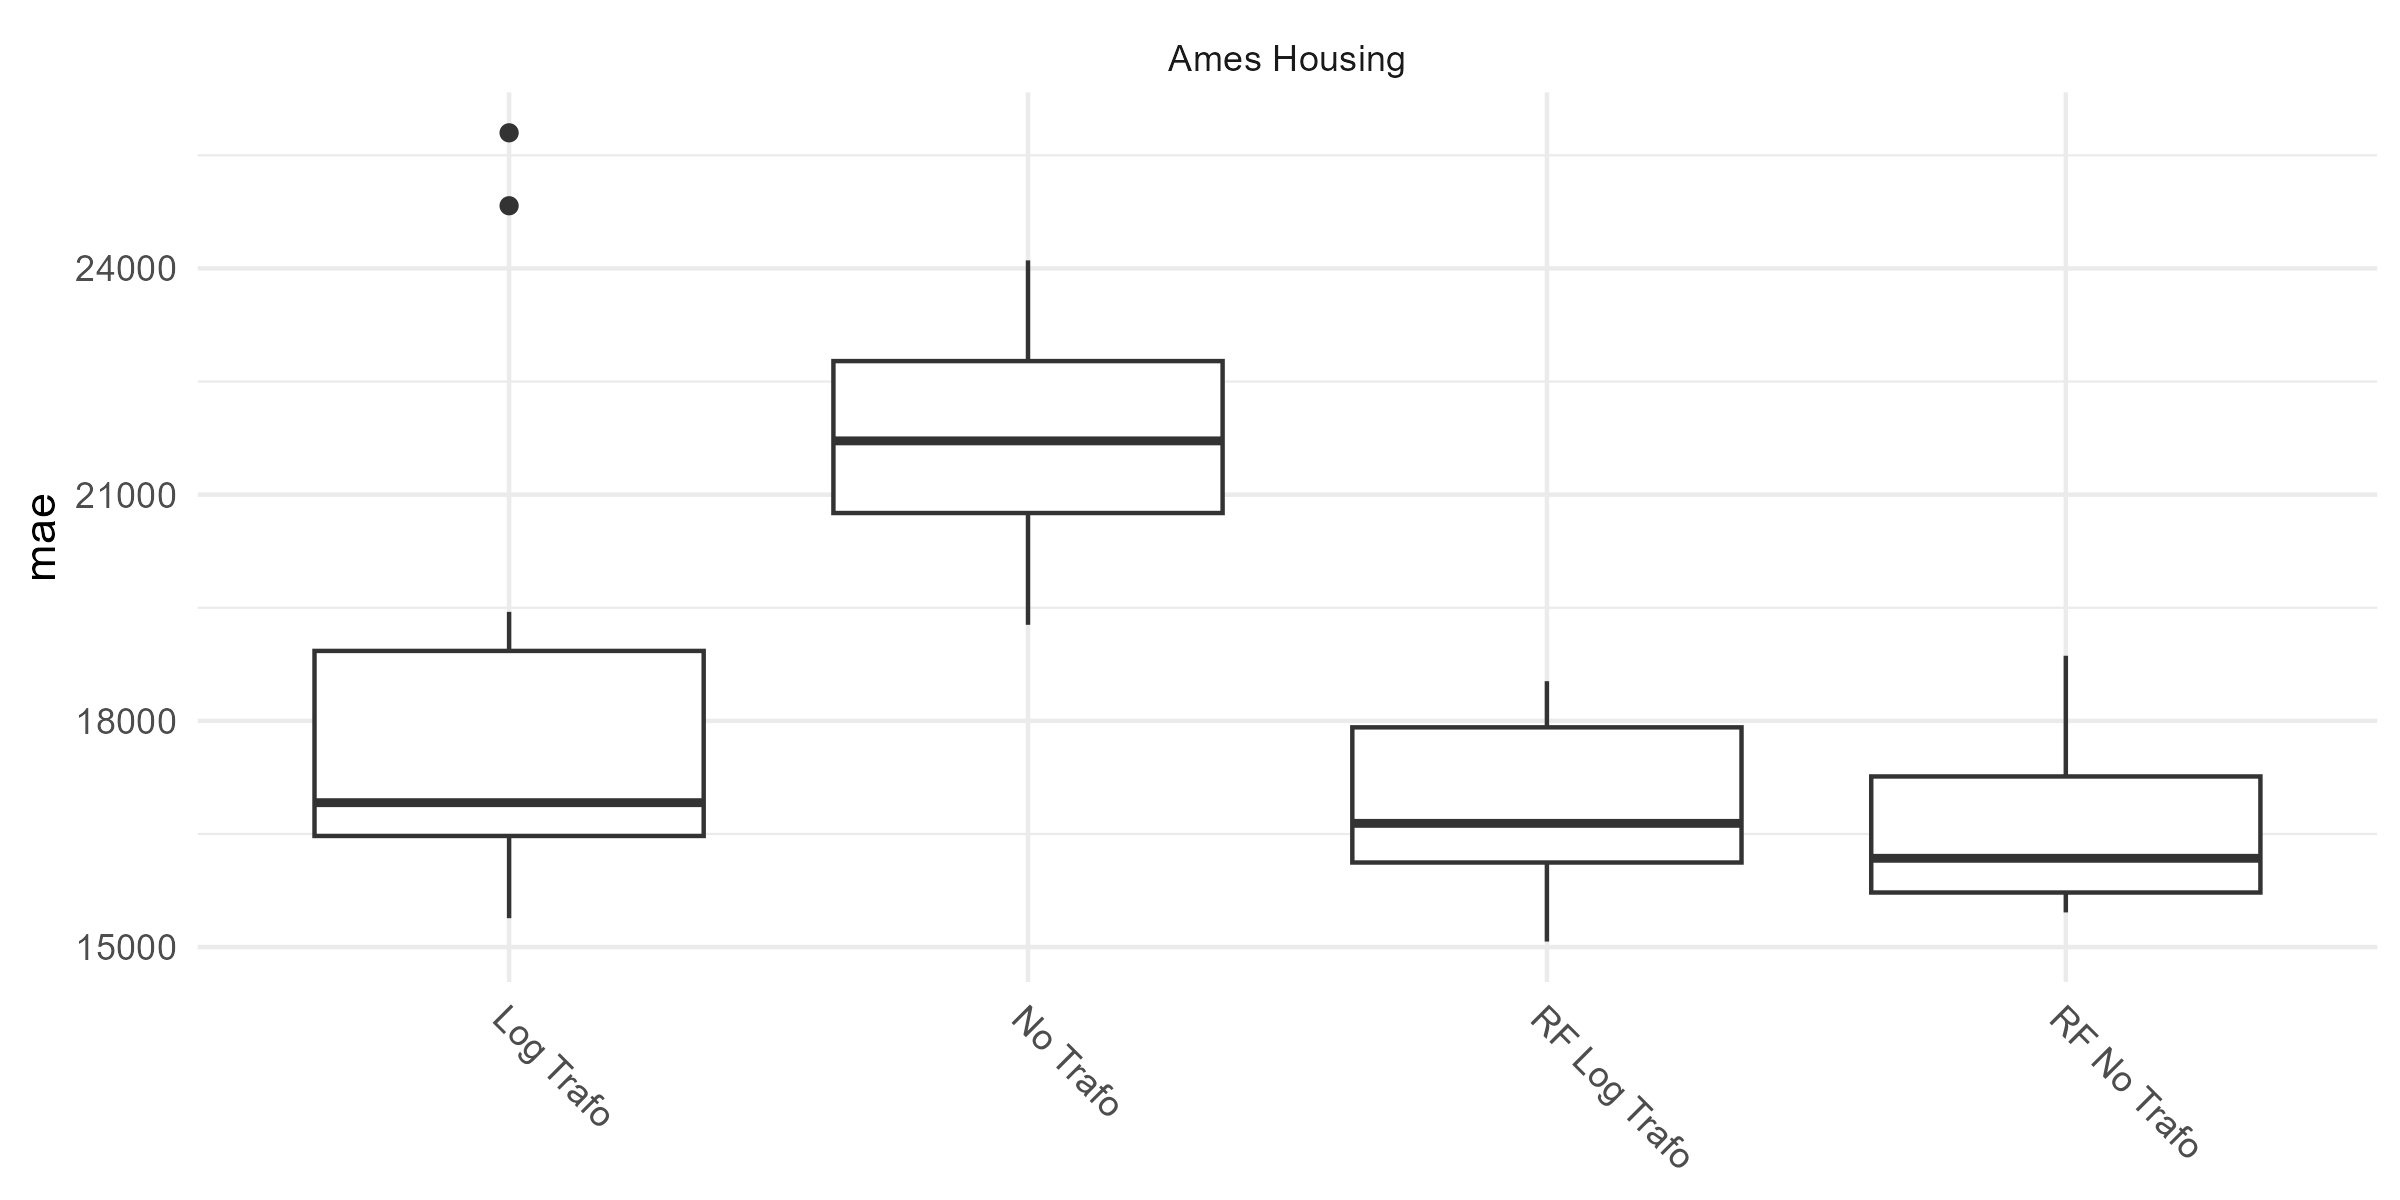
\includegraphics[width=\textwidth]{figure/01_transformation_comparison_all_algorithms.png}
\vspace{-0.3em}

\scriptsize
Ames housing data, 10-fold CV, MAE.
\end{column}
\begin{column}{0.46\textwidth}
\vspace{0.3em}
Log-transforming the target substantially improves the linear model but barely changes random forest.

\vspace{0.5em}
\textbf{Practical takeaway:}
\begin{itemize}\setlength{\itemsep}{3pt}
    \item Linear and distance-based models benefit most
    \item Tree-based models can fit skewed targets natively (split thresholds adapt to the data); gradient boosting or random forests often do not need a target transform
    \item Always benchmark with vs.\ without to verify it helps
\end{itemize}
\end{column}
\end{columns}
\end{vbframe}


\begin{vbframe}{Summary}
\vfill
\begin{itemize}
    \item Skewed targets cause heteroscedastic errors that hurt models with squared-error loss
    \item Common target transformations: $\log(y)$, $\log(y+1)$, Box-Cox ($y > 0$), Yeo-Johnson (any $y$)
    \item The transformation is part of the model pipeline (transform $\rightarrow$ fit $\rightarrow$ invert), not a preprocessing step -- parameters must be estimated per fold to avoid leakage
    \item Tree-based models adapt their splits to the target distribution and rarely benefit from a target transform; the benefit is greatest for linear and distance-based models
    \item The same principle applies to \textbf{detrending in time series}: subtract a trend (target transformation), model residuals, add the trend back at prediction time $\rightarrow$ see time series chapter
\end{itemize}
\vfill
\end{vbframe}


\endlecture
\end{document}
